\documentclass[sigconf,nonacm]{acmart}

\AtBeginDocument{%
  \providecommand\BibTeX{{%
    Bib\TeX}}}
\begin{document}

\title{Prenova Urnika Fakultete - Končno Poročilo}

\author{Nik Čadež}
\affiliation{
  \institution{University of Ljubljana, Faculty of Computer and Information Science}
  \city{Ljubljana}
  \country{Slovenia}}
\email{nc3408@student.uni-lj.si}

\author{Nik Jukič}
\affiliation{
  \institution{University of Ljubljana, Faculty of Computer and Information Science}
  \city{Ljubljana}
  \country{Slovenia}}
\email{nj7322@student.uni-lj.si}

\author{Gašper Kolbezen}
\affiliation{
  \institution{University of Ljubljana, Faculty of Computer and Information Science}
  \city{Ljubljana}
  \country{Slovenia}}
\email{gk9956@student.uni-lj.si}

%%
%% The abstract is a short summary of the work to be presented in the
%% article.
\begin{abstract}
In this report, we present the redesign of the Faculty of Computer and Information Science schedule, focusing on improving the user experience, especially on mobile devices. The project included user needs research, prototyping, usability testing, and iterative design refinement. The result is a high-fidelity prototype developed in Figma, featuring intuitive navigation, schedule customization for users, and integration with the online classroom. During development, we emphasized the importance of a user-centered approach and interactive testing, which significantly contributed to shaping the final product.
\end{abstract}

%% Keywords. The author(s) should pick words that accurately describe
%% the work being presented. Separate the keywords with commas.
\keywords{HCI, UI, Graphic Design, Prototyping, Figma, Usability Testing, A/B testing}
%% A "teaser" image appears between the author and affiliation
%% information and the body of the document, and typically spans the
%% page.

%%
%% This command processes the author and affiliation and title
%% information and builds the first part of the formatted document.
\maketitle

\section{Introduction}
As part of the Human-Computer Interaction course, we undertook the redesign of the Faculty of Computer and Information Science schedule system. The motivation for this project stemmed from user dissatisfaction with the current implementation, which is only available as a web application and is not suitable for mobile devices. The goal of the redesign was to develop an application that would improve the student experience, particularly on mobile devices, while maintaining most of the core functionalities and extending them with new features that users expressed interest in having in their timetable. With a strong focus on creating a beautiful and intuitive design, we aimed to transform the scheduling experience into something both functional and visually appealing. This report presents the key project phases, from research and prototype design to testing and implementation of solutions.

\section{Methodology}
For this project, we implemented the user-centered design methodology as taught in our Human-Computer Interaction lectures. This systematic approach, which emphasizes iterative design and user involvement throughout the development process, provided us with a structured framework for addressing the schedule redesign challenge. The following sections detail how we applied these theoretical concepts in practice, from initial user research through to final implementation.

\subsection{Project Proposal}
At the beginning of the project, we created a project proposal \cite{predlog}, in which we outlined the project's course and objectives. These were selected based on our own experiences with the current schedule implementation and focused on mobile device adaptation, improved navigation, and schedule personalization for users. Based on the initial ideas, we mapped out a user experience hierarchy \cite{hierarhija}, which helped us determine the initial goals and functionalities for our project. We decided that during the redesign, we would gather feedback almost exclusively from faculty students, as the redesign is primarily intended for their use.

\subsection{Collecting Student Feedback}
In the initial phase of our redesign process, we conducted a comprehensive survey \cite{anketa1} to understand our users better. The survey's primary objectives were to gather student feedback on the existing schedule implementation, identify desired changes and functionalities, and collect data about students' calendar preferences and usage patterns.

The survey, completed by 20 students, provided valuable insights into our user base and their interaction patterns with calendar applications. A significant finding revealed that 80% of respondents primarily access the schedule on their mobile devices, validating our decision to prioritize the mobile view. The results also highlighted several key user requirements, including the ability to select lab and lecture time slots, and integration with the online classroom platform for activity display. Additionally, we discovered that approximately one-third of students export their schedules to external calendars, with nearly half either actively using or expressing a preference for Google Calendar's interface.

Given the strong preference for Google Calendar among our respondents, we strategically decided to incorporate elements of its design principles and gesture-based interactions into our solution. This approach leverages users' familiarity with established calendar interfaces while addressing their specific needs. The complete survey results are available in the portfolio \cite{anketa1-rez}.

Building on these insights, we developed a detailed user persona \cite{userpersona} and corresponding empathy map \cite{empathymap}. These tools helped us establish fundamental design principles \cite{principi} that would guide our product development, ensuring alignment with user needs and preferences.

Based on the comprehensive analysis of our survey responses, combined with the insights derived from our user persona and empathy mapping exercises, we were able to distill our findings into actionable design principles. This systematic approach to transforming raw user feedback into structured guidelines ensured that no crucial user insights were lost in the process. The following key principles emerged as fundamental pillars that would serve as our decision-making framework throughout the development process.

\subsubsection{\textbf{Identified Key Principles}}
\begin{itemize}
\item \textbf{Organization:} The schedule interface must provide comprehensive daily, weekly, and monthly viewing options. Related academic components (lectures and practical sessions) of the same course shall maintain consistent color coding. The system must facilitate efficient filtering of courses by academic year and faculty members.
\item \textbf{Visual Coherence:} Implementation of a carefully curated color scheme is essential, ensuring optimal contrast and visual hierarchy. Related course components must share identical color coding to enhance intuitive recognition and improve information grouping.
\item \textbf{Intuitive Interface:} The schedule must provide a user-friendly experience with clear, logical interaction patterns that minimize the learning curve for new users while maintaining efficiency for regular users.
\item \textbf{Labeling:} Course sessions must feature clear, unambiguous identifiers, utilizing both full names and standardized abbreviations. Filter mechanisms must implement precise, self-explanatory options to prevent user error.
\item \textbf{Navigation:} The system must provide enhanced navigation efficiency compared to the current implementation. Users' personal schedules shall serve as the default landing page, with streamlined access for quick returns to this view.
\item \textbf{Search Functionality:} The platform must incorporate a comprehensive search system encompassing courses, faculty members, and time slots.
\item \textbf{Customization:} Users must have the capability to select and customize their preferred lecture and practical session attendance schedules.
\item \textbf{Information Architecture:} Each schedule view must implement progressive disclosure principles, presenting only contextually relevant information to maintain clarity and reduce cognitive load.
\end{itemize}

\subsection{Prototyping}

Our course exercises included a crucial prototyping phase focused on developing the final product's visual concept. The complete collection of low-fidelity prototypes can be found in the portfolio~\cite{prototyping}. Initially, we created paper sketches of the application's login page and schedule view, incorporating essential functionality buttons intended for the final product. These prototypes underwent an iterative feedback process with fellow students.

\noindent
The evolution of our design showed interesting patterns. While the login page remained relatively stable with minor adjustments, the main view experienced significant transformations across iterations. The first version was notably basic, displaying only individual subjects without any navigation elements. This limitation, along with the absence of time indicators on the calendar's edge, was quickly identified as an area for improvement.

\noindent
Responding to initial feedback, our second iteration brought several enhancements:
\begin{itemize}
    \item Added hourly time markers for clearer schedule visualization
    \item Implemented color coding for different subjects
    \item Included detailed information within schedule blocks (subject details, classroom locations, and session types)
    \item Incorporated basic navigation elements and date indicators
\end{itemize}

\noindent
Though this version received more favorable feedback, users highlighted two main concerns: confusing button labels and a desire for activity notifications.

\noindent
The third iteration addressed these issues directly by:
\begin{itemize}
    \item Implementing activity notification features
    \item Refining button labels for clarity
    \item Adding menus for exercise time slot selection
\end{itemize}

\noindent
Key feedback points from the prototyping process included:
\begin{itemize}
    \item Satisfaction with the prototype's appearance
    \item Desires for search capabilities across all possible entries
    \item Unclear selected buttons and their labels
    \item Wish for more intuitive navigation
\end{itemize}

\noindent
With the low-fidelity prototype completed and refined through multiple iterations, we established a solid foundation for developing a high-fidelity prototype using Figma.

\begin{figure}[h]
  \centering
  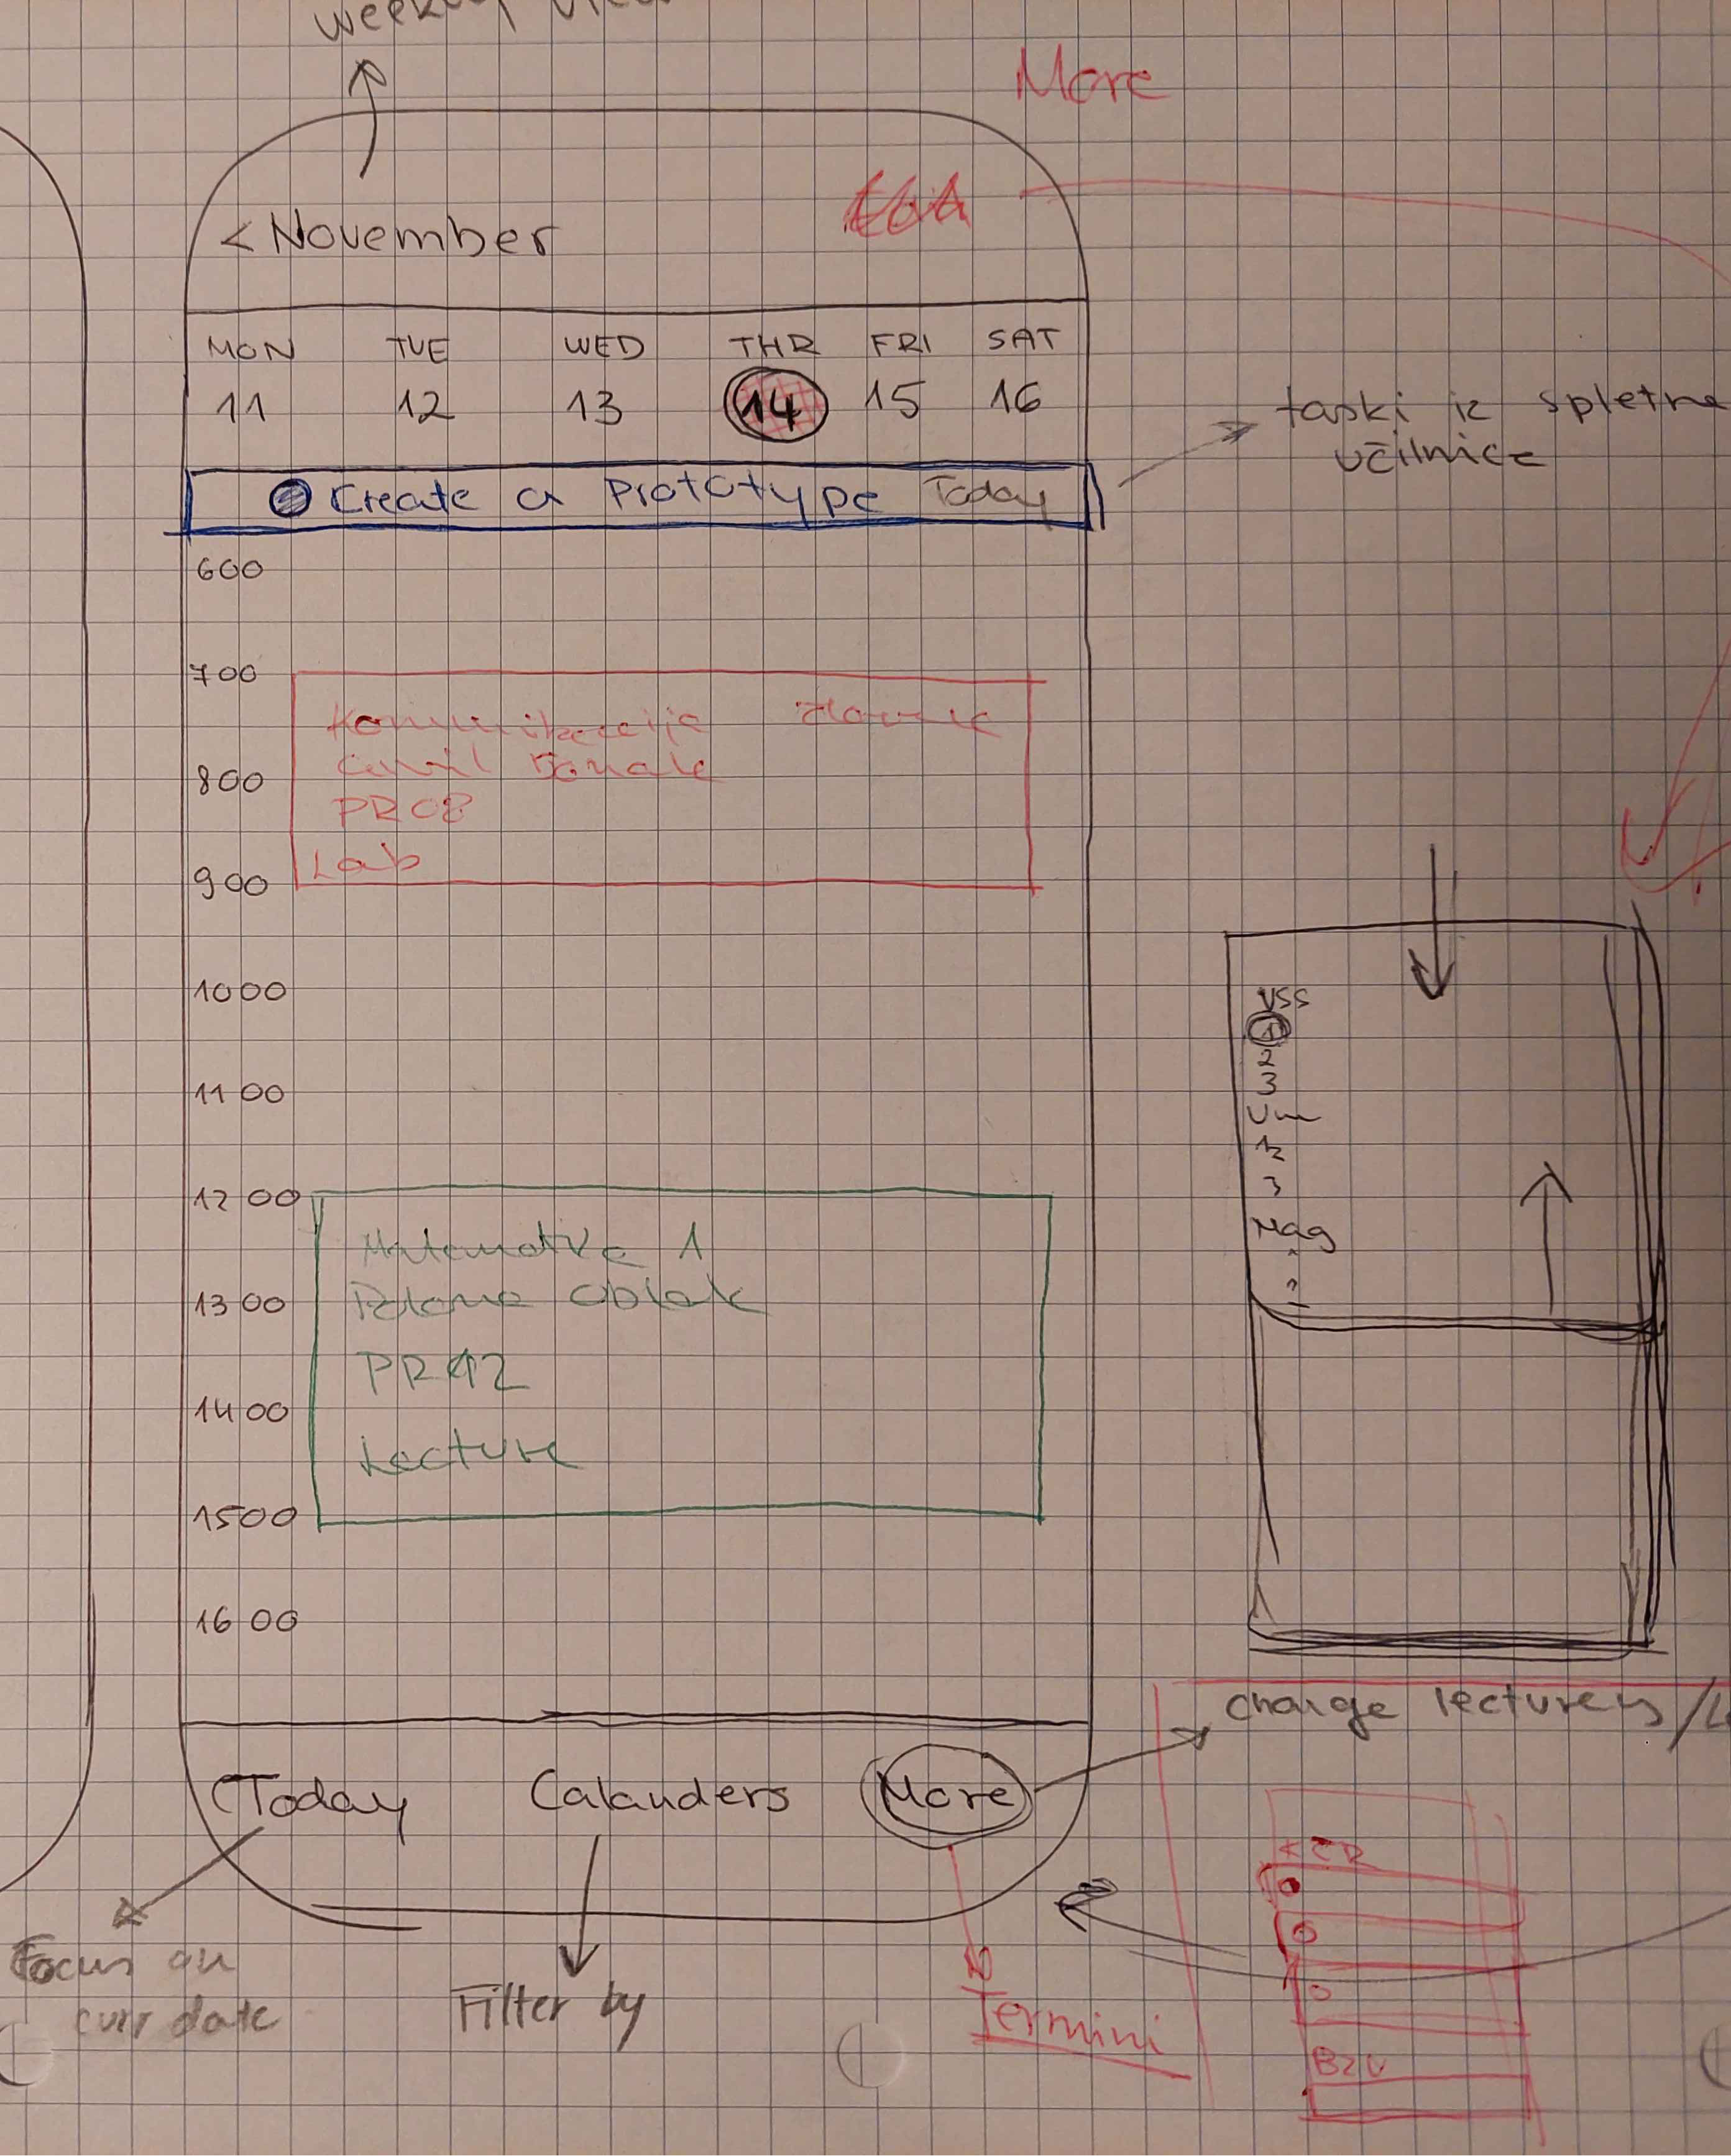
\includegraphics[width=\linewidth]{low-fidelity-prototype.png}
  \caption{Final low-fidelity prototype, created as part of prototyping}
\end{figure}

\subsection{Creating a High-Fidelity Prototype in Figma}
Following the development of our low-fidelity prototype and incorporating the feedback received during the prototyping phase, we proceeded to create a high-fidelity prototype using Figma, a powerful tool for developing interactive user interfaces.

The process began with the creation of a user flow map \cite{jouneymap}, which established the foundation for our application's functional design. Within Figma, we developed eight comprehensive screen masks for various user flows, all of which are documented in the portfolio \cite{figma1}:

\begin{itemize}
\item \textbf{Login:} A streamlined sign-in page offering authentication options through either user accounts or digital identity.
\item \textbf{Weekly and monthly view, plus two day views:} Multiple schedule display options, including monthly, weekly, and daily views, with one daily view specifically demonstrating overlapping appointment handling.
\item \textbf{Subject search:} A comprehensive view displaying the complete list of available subjects.
\item \textbf{Menu for selecting exercise and lecture slots:} An intuitive menu interface for selecting exercise and lecture time slots.
\item \textbf{View selection menu:} A versatile menu system enabling searches by various categories: subjects, professors, classrooms, and groups.
\end{itemize}

During the screen mask development process, we proactively created a concise accessibility improvement plan \cite{dostopnost}. This approach ensured adherence to best practices from the outset, eliminating the need for significant modifications later. Based on prototyping feedback, we retained the fundamental layout of the high-fidelity prototype, including the activity notification feature integrated with the online classroom. We also maintained the quick-access buttons for returning to daily view and navigating to monthly view. However, we implemented strategic modifications, replacing the "More" and "Calendars" buttons with logout functionality and dedicated menus for category search and time slot selection.

\begin{figure}[h]
  \centering
  \includegraphics[width=\linewidth]{dnevni-pogled.png}
  \caption{Version one of the daily schedule view, created in Figma}
\end{figure}

\subsection{Usability Testing}
As part of the course exercises, we conducted usability testing to evaluate our prototype's effectiveness. The testing served multiple purposes: to assess users' ability to perform key tasks, measure task completion efficiency, and gather feedback on the prototype's interaction design. We also used this opportunity to compare different user interface elements, specifically focusing on two variations of the time slot selection menu and the visual presentation of schedule lines. Furthermore, we sought user feedback regarding the potential inclusion of a wheel-based options menu, with these interface variations documented in the portfolio \cite{figma1}.

The usability testing consisted of five distinct tasks, with each participant beginning from the login page:

\begin{itemize}
\item View your schedule.
\item Change the exercise time slot.
\item View the schedule without logging in.
\item Open the monthly schedule view.
\item Open the schedule for the Human-Computer Interaction course.
\end{itemize}

To evaluate task performance comprehensively, we measured four key parameters:

\begin{itemize}
\item Task completion success/failure
\item Number of clicks required
\item Task completion time
\item Number of incorrect clicks
\end{itemize}

All test results were documented and are available in the portfolio \cite{testing}. The subsequent analysis revealed several significant findings. Overall, the prototype demonstrated strong performance, with users completing tasks efficiently despite their unfamiliarity with the interface. However, we identified a notable usability issue with the "Views" button. While intended to access a menu for filtering by courses, professors, classrooms, and groups, users frequently mistook it for the monthly schedule view access point.

User feedback provided clear direction for interface improvements. Participants expressed a preference for simpler navigation over the proposed wheel-based options menu. Regarding the schedule display, users favored the inclusion of lines but suggested making them thinner than our initial design. The time slot selection menu was more effective with clearly defined buttons. While users responded positively to the overall redesign, they highlighted several desired enhancements: more distinctive buttons, the addition of activity duration in notifications, and the implementation of a general search functionality.

\subsection{High-fidelity Prototype Iteration}
Following the usability testing feedback, we implemented several significant improvements to the prototype. The most notable enhancement was the introduction of a sidebar menu, strategically placed with its access button in the top-left corner. This new sidebar now houses the previously scattered functionalities, including options to toggle between daily, weekly, or monthly views, as well as search capabilities for courses, professors, classrooms, and groups. This replacement of the previous time-view navigation button has proven more intuitive and user-friendly.

The sidebar's integrated search function now spans all categories, effectively addressing the confusion caused by unclear buttons in the previous design. This modification was inspired by popular applications' navigation patterns, making it naturally discoverable for users seeking specific features. The streamlined main view now displays only essential buttons: current day navigation, logout, and time slot selection, along with a newly added schedule export function. This reorganization has not only simplified the interface but also optimized the available space.

Color scheme optimization was a crucial aspect of our iteration process. We developed multiple color palettes, each thoughtfully designed with accessibility in mind, particularly for users with color blindness. These included a base version with pastel colors, blue-centric and red-centric schemes, and a blue-yellow combination. Each palette underwent careful contrast adjustments and text color optimization to ensure readability.

The university's signature red color was explored as a design element for the toolbars, resulting in various implementations. We experimented with partial and full toolbar coloring, as well as different sidebar color treatments. The top-right corner underwent multiple iterations for the user controls, exploring different combinations of elements such as a settings wheel, search bar, and logout button. Additionally, we developed an alternative login page design. All these design variations are documented in detail in the portfolio \cite{brainstorming}.

\begin{figure}[h]
  \centering
  \includegraphics[width=\linewidth]{side-menu.png}
  \caption{Implementation of the side menu in Figma}
\end{figure}

\subsection{Second Round of User Feedback}
After completing the second iteration of our high-fidelity prototype, we found ourselves with multiple user interface variations. This diversity emerged from our brainstorming sessions, where we strived to implement the most effective UI based on our understanding of user requirements. With several promising options at hand, we recognized the need for additional user feedback to make informed decisions.

To gather this crucial feedback, we designed a second survey \cite{anketa2} that focused on two core aspects. The first component involved A/B testing between different UI design options, allowing us to directly compare user preferences. The second component centered on color accessibility, particularly focusing on creating an inclusive experience for colorblind users. Understanding the critical role that colors play in user interface design, we were committed to developing an experience that would be equally effective and enjoyable for all users, including those requiring special accessibility features.

Our survey garnered 17 responses, with detailed results available in the portfolio \cite{anketa2-rez}. Initially, we screened participants for color blindness, though all respondents reported having normal color vision. The survey progressed through several sections, beginning with questions about element placement and a comparative analysis of two login page designs, followed by inquiries about color palettes, contrast preferences, and the potential use of red in toolbars.

The results regarding color palettes were notably decisive, with most questions receiving near-unanimous responses, which simplified our implementation decisions. Only two areas showed closer competition: contrast preferences and sidebar coloring. In these instances, we opted to implement the marginally preferred options, particularly as they aligned well with other design choices. Notably, the proposed red toolbar option received no support across all questions.

The most valuable insights emerged from the toolbar-related questions. Respondents strongly favored incorporating a search function in the top toolbar and relocating the logout button to the side menu. However, during implementation, we encountered a practical limitation: the front camera placement on modern smartphones would interfere with centrally positioned elements in the top toolbar. This technical constraint led us to maintain the search function exclusively in the side toolbar. Nevertheless, we proceeded with moving the logout button to the side menu, replacing it with a "Back" button—a change that ultimately enhanced the application's navigation efficiency.

\begin{figure}[h]
  \centering
  \includegraphics[width=.3\linewidth]{login v1.png}\hfill
            \includegraphics[width=.3\linewidth]{login2.png}\hfill
            \includegraphics[width=.3\linewidth]{login.png}\hfill
  \caption{Iteracija prijavne strani}
\end{figure}

\section{Results}

The project successfully culminated in a comprehensive redesign of the Faculty's schedule system, with several notable achievements:

\subsection{Final Design Implementation}

The final product consists of a high-fidelity interactive prototype developed in Figma \cite{figma-link}, comprising ten interconnected screen views with functional transitions that simulate real application behavior. The prototype effectively addresses the initial project objectives while incorporating user feedback from multiple testing phases.

\subsection{Key Features Implemented}

\subsubsection{Intuitive Navigation System}
\begin{itemize}
    \item Implementation of a streamlined sidebar menu
    \item Quick access to daily, weekly, and monthly views
    \item Integrated search functionality across all categories
\end{itemize}

\subsubsection{Enhanced User Interface}
\begin{itemize}
    \item Optimized color schemes with accessibility considerations
    \item Clear visual hierarchy and consistent design language
    \item Responsive layout suitable for mobile devices
\end{itemize}

\subsubsection{Improved Functionality}
\begin{itemize}
    \item Schedule customization options
    \item Exercise and lecture time slot selection
    \item Integration with the online classroom
    \item Schedule export capabilities
\end{itemize}

\subsection{Design Optimizations}

The final design incorporates several refinements based on user testing and feedback:

\begin{itemize}
    \item Simplified navigation structure with consolidated menu options
    \item Optimized placement of key functions for improved usability
    \item Carefully selected color palettes ensuring accessibility
    \item Improved contrast ratios for better readability
    \item Strategic placement of interface elements accounting for modern smartphone designs
\end{itemize}

\subsection{Future Potential}

The project has laid a strong foundation for potential future development, with the design work serving as a valuable reference for any subsequent implementation of the schedule system. While actual development was beyond the project's scope, the detailed design specifications and user research provide a solid basis for future implementation efforts.

The final prototype represents a significant improvement over the existing system, particularly in terms of mobile usability, user experience, and functionality, meeting the primary objectives established at the project's outset.
\bibliographystyle{ACM-Reference-Format}
\bibliography{sample-base}
\end{document}
\endinput
